% ------------------------------------------------------------------------------
% TYPO3 Version 10.3 - What's New (Dutch Version)
%
% @license	Creative Commons BY-NC-SA 3.0
% @link		https://typo3.org/help/documentation/whats-new/
% @language	Dutch
% ------------------------------------------------------------------------------

\section{Wijzigingen voor integrators}
\begin{frame}[fragile]
	\frametitle{Wijzigingen voor integrators}

	\begin{center}\huge{Hoofdstuk 2:}\end{center}
	\begin{center}\huge{\color{typo3darkgrey}\textbf{Wijzigingen voor integrators}}\end{center}

\end{frame}

% ------------------------------------------------------------------------------
% Feature | 90333 | Dashboard

\begin{frame}[fragile]
	\frametitle{Wijzigingen voor integrators}
	\framesubtitle{Dashboard}

	% decrease font size for code listing
	\lstset{basicstyle=\tiny\ttfamily}

	\begin{itemize}
		\item Dashboard \textit{voorinstellingen} kunnen geconfigureerd worden voor nieuwe gebruikers of voor gebruikers
			die alle dashboards verwijderd hebben.
		\item Dit kan gebruikt worden om een "Snelstart" dashboard als standaard te tonen.
		\item Voorbeeld TSconfig:

\vspace{-0.4cm}
\begin{lstlisting}
options.dashboard.dashboardPresetsForNewUsers = default, dashboardPreset-myPreset
\end{lstlisting}

		\item Meerdere dashbooard-voorinstellingen kunnen gedefinieerd worden in een kommagescheiden lijst.

	\end{itemize}

\end{frame}

% ------------------------------------------------------------------------------
% Important | 89992 | Use New TranslationServer

\begin{frame}[fragile]
	\frametitle{Wijzigingen voor integrators}
	\framesubtitle{Platform voor beheer van vertalingen}

	\begin{itemize}
		\item De SaaS-oplossing "\href{https://crowdin.com/}{Crowdin}" wordt nu gebruikt als
			het platform voor het beheer van vertalingen voor TYPO3.
		\item We moedigen iedereen aan mee te doen en de vertalingen te verbeteren.
		\item Crowdin van gebruikt worden om de labels van de TYPO3 core te vertaling
			maar ook die van TYPO3 extensies.
		\item Lees meer hierover in de
			\href{https://docs.typo3.org/m/typo3/reference-coreapi/master/en-us/ApiOverview/Internationalization/TranslationServer/Crowdin.html}{TYPO3 documentatie}.
	\end{itemize}

	\begin{figure}
		
\includegraphics[width=0.40\linewidth]{ChangesForIntegrators/crowdin-logo.png}
	\end{figure}

\end{frame}

% ------------------------------------------------------------------------------
% Feature | 90266 | Fluid-based templated emails

\begin{frame}[fragile]
	\frametitle{Wijzigingen voor integrators}
	\framesubtitle{Fluid voor HTML e-mails (1)}

	% decrease font size for code listing
	\lstset{basicstyle=\smaller\ttfamily}

	\begin{itemize}
		\item TYPO3 ondersteunt nu het versturen van HTML en tekst e-mails op basis van sjablonen.
		\item E-mails worden gebouwd met Fluid sjablonen.
		\item E-mailsjablonen kunnen aangepast worden door de paden naar de sjabloonbestanden te overschrijven:

\vspace{-0.4cm}
\begin{lstlisting}
$GLOBALS['TYPO3_CONF_VARS']['MAIL']['templateRootPaths'][700] =
  'EXT:my_site_extension/Resources/Private/Templates/Email';

$GLOBALS['TYPO3_CONF_VARS']['MAIL']['layoutRootPaths'][700] =
  'EXT:my_site_extension/Resources/Private/Layouts';
\end{lstlisting}

	\end{itemize}

\end{frame}

% ------------------------------------------------------------------------------
% Feature | 90266 | Fluid-based templated emails

\begin{frame}[fragile]
	\frametitle{Wijzigingen voor integrators}
	\framesubtitle{Fluid voor HTML e-mails (2)}

	\begin{itemize}
		\item E-mail gebaseerd op Fluid-sjablonen worden bijvoorbeeld bij de volgende componenten gebruikt:

			\begin{itemize}
				\item Install Tool test e-mail (zie voorbeeld op volgende dia).
				\item Werkruimtenotificaties bij stadiumwijziging.
				\item Notificaties bij het inloggen van backend-gebruikers.
			\end{itemize}

	\end{itemize}

\end{frame}

% ------------------------------------------------------------------------------
% Feature | 90266 | Fluid-based templated emails

\begin{frame}[fragile]
	\frametitle{Wijzigingen voor integrators}
	\framesubtitle{Fluid voor HTML e-mails (3)}

	Test-e-mail verstuurd door de Install Tool:

	\begin{figure}
		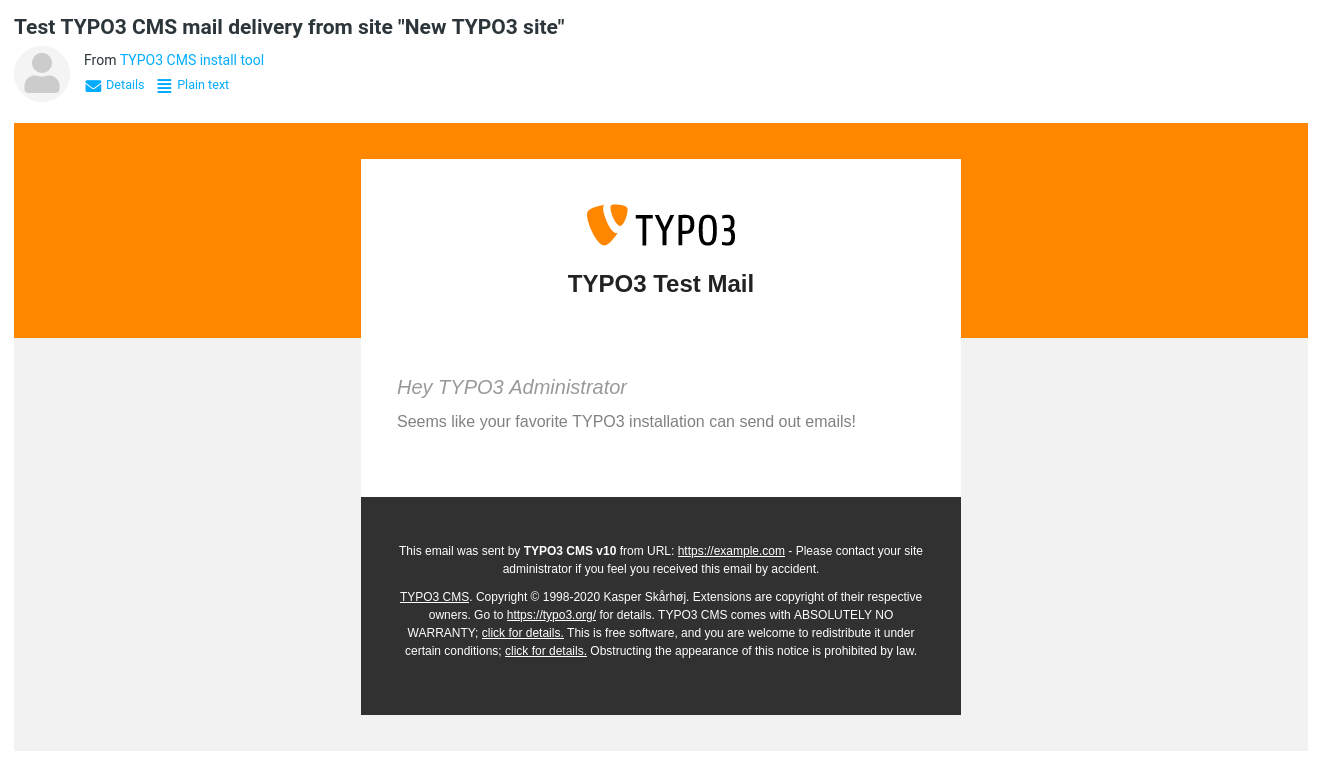
\includegraphics[width=0.8\linewidth]{ChangesForIntegrators/90266-FluidBasedTemplatedEmails.png}
	\end{figure}

\end{frame}

% ------------------------------------------------------------------------------
% Feature | 90203 | Make workspace available in TypoScript conditions

\begin{frame}[fragile]
	\frametitle{Wijzigingen voor integrators}
	\framesubtitle{Werkruimtes en TypoScript}

	% decrease font size for code listing
	\lstset{basicstyle=\smaller\ttfamily}

	\begin{itemize}
		\item Een nieuwe variabele voor de expressietaal is toegevoegd: \texttt{workspace}.
		\item Deze variabele kan in vergelijkingen gebruikt worden met gebruikelijke parameters van werkruimtes.
		\item Momenteel worden de volgende parameters ondersteund:\newline
			\small
				\texttt{workspaceId}, \texttt{isLive}, and \texttt{isOffline}.
			\normalsize
		\item Voorbeeld:

\vspace{-0.4cm}
\begin{lstlisting}
[workspace.workspaceId === 3]
  # Huidige werkruimte ID is 3
[end]
\end{lstlisting}

	\end{itemize}

\end{frame}

% ------------------------------------------------------------------------------
% Feature | 88962 | Re-implement old PIDupinRootline TypoScript condition

\begin{frame}[fragile]
	\frametitle{Wijzigingen voor integrators}
	\framesubtitle{TypoScript}

	% decrease font size for code listing
	\lstset{basicstyle=\smaller\ttfamily}

	\begin{itemize}
		\item De oude \texttt{PIDupinRootline} voorwaarde is opnieuw geïmplementeerd
			in TypoScript met de Symfony uitdrukkingstaal.
		\item Syntax van oude TypoScript voorwaarde:

\vspace{-0.4cm}
\begin{lstlisting}
[PIDupinRootline = 30]
  page.10.value = Ik ben op een subpagina van pagina met UID 30.
[END]
\end{lstlisting}

		\item Nieuwe syntax TypoScript voorwaarde:

\vspace{-0.4cm}
\begin{lstlisting}
[30 in tree.rootLineParentIds]
  page.10.value = Ik ben op een subpagina van pagina met UID 30.
[END]
\end{lstlisting}

	\end{itemize}

\end{frame}

% ------------------------------------------------------------------------------
% Feature | 90426 | Browser-native lazy loading for images

\begin{frame}[fragile]
	\frametitle{Wijzigingen voor integrators}
	\framesubtitle{Vertraagd laden van afbeeldingen}

	% decrease font size for code listing
	\lstset{basicstyle=\smaller\ttfamily}

	\begin{itemize}
		\item Het HTML attribuut \texttt{loading} kan ingesteld worden bij \texttt{<img>}-tags.
		\item Browsers die dit ondersteunen zullen de afbeeldingen pas laden als ze zichtbaar worden.
		\item Dit gedrag kan gewijzigd worden met de volgende TypoScript constante:

\vspace{-0.4cm}
\begin{lstlisting}
styles.content.image.lazyLoading = lazy
\end{lstlisting}

		\item Geldige waarden zijn: \texttt{lazy} (default), \texttt{eager}, and \texttt{auto}.
		\item De Fluid \textit{Image-ViewHelper} ondersteunt ook vertraagd laden:

\vspace{-0.4cm}
\begin{lstlisting}
<f:image src="{fileObject}" treatIdAsReference="true"
  loading="lazy" />
\end{lstlisting}

	\end{itemize}

\end{frame}

% ------------------------------------------------------------------------------
% Important | 89869 | Change lockIP default to disabled for both frontend and backend

\begin{frame}[fragile]
	\frametitle{Wijzigingen voor integrators}
	\framesubtitle{Standaard waarden voor \texttt{lockIP}/\texttt{lockIPv6}}

	% decrease font size for code listing
	\lstset{basicstyle=\smaller\ttfamily}

	\begin{itemize}
		\item De standaardinstellingen voor \texttt{lockIP} zijn veranderd.
		\item De volgende vier systeemvariabelen zijn nu standaard \textbf{uitgeschakeld}:

			\begin{itemize}
				\item \texttt{[FE]['lockIP']}
				\item \texttt{[FE]['lockIPv6']}
				\item \texttt{[BE]['lockIP']}
				\item \texttt{[BE]['lockIPv6']}
			\end{itemize}

		\item De oude standaardwaarden ("\texttt{4}" voor de backend en "\texttt{2}" voor de frontend)
			zorgden voor problemen bij bezoekers met IPv4 en IPv6 ondersteuning.

	\end{itemize}

\end{frame}

% ------------------------------------------------------------------------------
% Feature | 90052 | Form YAML configuration available in configuration module

\begin{frame}[fragile]
	\frametitle{Wijzigingen voor integrators}
	\framesubtitle{Formulieren: YAML configuratie}

	\begin{columns}[T]
		\begin{column}{.04\textwidth}
		\end{column}
		\begin{column}{.38\textwidth}

			Als de systeemextensie \texttt{EXT:form} is geïnstalleerd kan de YAML-configuratie
			getoond worden onder \textbf{SYSTEEM} $\rightarrow$ \textbf{Configuratie}.

			\vspace{0.2cm}

			Admins moeten natuurlijk ook \texttt{EXT:lowlevel} geïnstalleerd hebben.

		\end{column}
		\begin{column}{.58\textwidth}
			\vspace{-0.3cm}
			\begin{figure}
				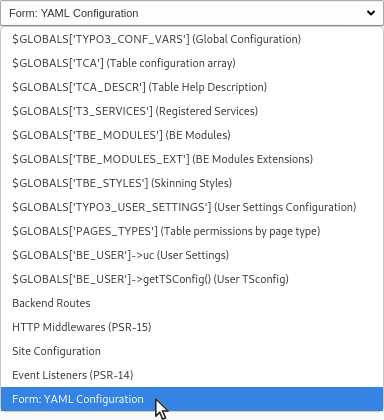
\includegraphics[width=0.70\linewidth]{ChangesForIntegrators/90052-AddYamlConfigurationToConfigurationModule.png}
			\end{figure}
		\end{column}
	\end{columns}

\end{frame}

% ------------------------------------------------------------------------------
% Feature | 88147 | Add possibility to configure the path to sitemap xslFile

\begin{frame}[fragile]
	\frametitle{Wijzigingen voor integrators}
	\framesubtitle{SEO: \texttt{Sitemap.xsl}}

	% decrease font size for code listing
	\lstset{basicstyle=\tiny\ttfamily}

	\begin{itemize}
		\item Het standaardpad naar het bestand \texttt{Sitempa.xsl} van de systeemextensie
			\texttt{EXT:seo} kan nu aangepast worden:

\vspace{-0.4cm}
\begin{lstlisting}
# Globaal voor alle sitemaps:
plugin.tx_seo.config.xslFile = EXT:myext/Resources/Public/CSS/mySite.xsl

# Voor alle sitemaps van een specifiek type:
plugin.tx_seo.config.<sitemapType>.sitemaps.xslFile = EXT:myext/Resources/Public/CSS/mySite.xsl

# Voor een specifieke sitemap:
plugin.tx_seo.config.<sitemapType>.sitemaps.<sitemap>.config.xslFile =
  EXT:myext/Resources/Public/CSS/mySite.xsl
\end{lstlisting}

		\item Het standaardpad is:\newline
			\smaller
				\texttt{EXT:seo/Resources/Public/CSS/Sitemap.xsl}
			\normalsize

	\end{itemize}

\end{frame}

% ------------------------------------------------------------------------------
% Feature | 82062 | Progress for Reference Index update on CLI

\begin{frame}[fragile]
	\frametitle{Wijzigingen voor integrators}
	\framesubtitle{Referentie-index}

	% decrease font size for code listing
	\lstset{basicstyle=\tiny\ttfamily}

	\begin{itemize}
		\item Bij het bijwerken van de referentie-index toont een balk de voortgang voor elke
			databasetabel.
	\end{itemize}

	\begin{figure}
		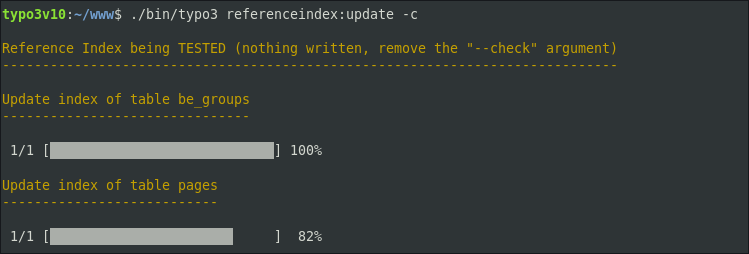
\includegraphics[width=0.85\linewidth]{ChangesForIntegrators/82062-ProgressForReferenceIndexUpdateOnCli.png}
	\end{figure}

\end{frame}

% ------------------------------------------------------------------------------
% Feature | 90425 | Add seo fields to info module

\begin{frame}[fragile]
	\frametitle{Wijzigingen voor integrators}
	\framesubtitle{Infomodule}

	\begin{itemize}
		\item SEO en Sociale Media-details zijn toegevoegd aan de Infomodule:\newline
			\textbf{WEB} $\rightarrow$ \textbf{Info} $\rightarrow$ \textbf{Overzicht paginaboom}.
	\end{itemize}

	\begin{figure}
		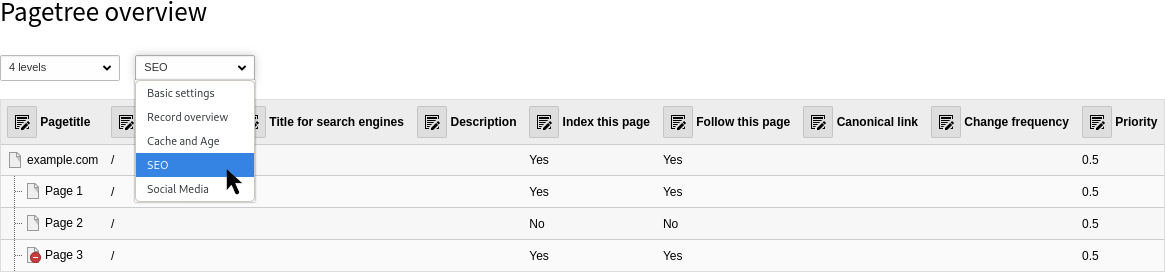
\includegraphics[width=0.85\linewidth]{ChangesForIntegrators/90425-AddSeoFieldsToInfoModule.png}
	\end{figure}

\end{frame}

% ------------------------------------------------------------------------------
% Feature | 59452 | scheduler:run command accepts multiple task options

\begin{frame}[fragile]
	\frametitle{Wijzigingen voor integrators}
	\framesubtitle{Taakplanner}

	% decrease font size for code listing
	\lstset{basicstyle=\tiny\ttfamily}

	\begin{itemize}
		\item Meerdere taken kunnen uitgevoerd worden met de optie \texttt{-}\texttt{-}\texttt{task}
	\end{itemize}

	\begin{figure}
		
\includegraphics[width=0.85\linewidth]{ChangesForIntegrators/59452a-MultipleTasksInSchedulerCommand.png}
	\end{figure}

	\begin{itemize}
		\item Uitgebreide uitvoer kan ingeschakeld worden met \texttt{-}\texttt{v} en \texttt{-}\texttt{vv}
	\end{itemize}

	\begin{figure}
		
\includegraphics[width=0.85\linewidth]{ChangesForIntegrators/59452b-MultipleTasksInSchedulerCommand.png}
	\end{figure}

\end{frame}

% ------------------------------------------------------------------------------
% Feature | 90298 | Improve user info in BE User module

\begin{frame}[fragile]
	\frametitle{Wijzigingen voor integrators}
	\framesubtitle{Module backend-gebruikers}

	\begin{itemize}
		\item Een nieuwe detailweergave van backend-gebruikers toont alle relevante data.
		\item Extra velden zijn toegevoegd aan de functie voor het vergelijken van gebruikers.
		\item Deze functie kijkt nu ook naar subgroepen.
		\item Het uiterlijk van de module zal verder aangepast en geoptimaliseerd worden.
		\item Deze wijzigingen maken het makkelijker om gebruikers te controleren en te
			vergelijken zonder naar de gebruiker over te schakelen.
	\end{itemize}

\end{frame}

% ------------------------------------------------------------------------------
% Feature | 89894 | Separate system extensions from 3rd-party extensions visually

\begin{frame}[fragile]
	\frametitle{Backend User Interface}
	\framesubtitle{Extensiebeheer}

	Systeemextensies en extensies van derden kunnen nu apart getoond worden in de module Extensies.

	\begin{figure}
		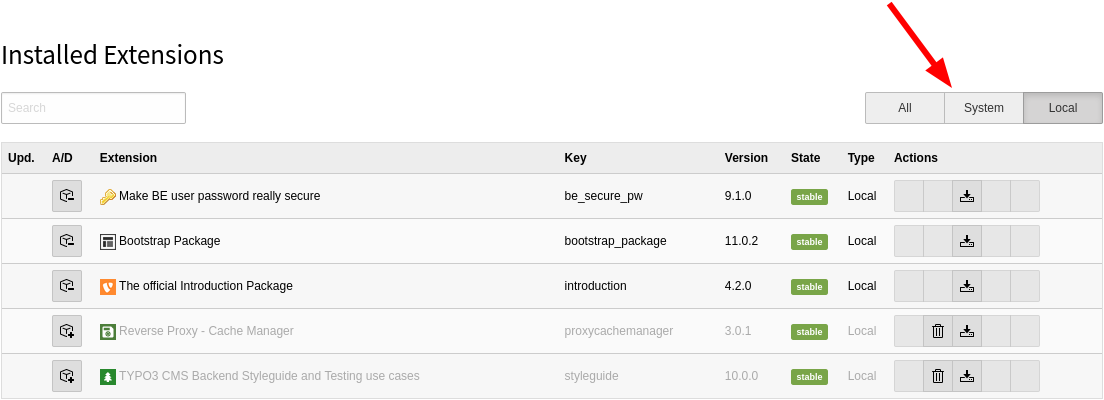
\includegraphics[width=0.9\linewidth]{BackendUserInterface/89894-SeparateSystemExtensionsFrom3rdPartyExtensionsVisually.png}
	\end{figure}

\end{frame}

% ------------------------------------------------------------------------------
% Feature | 90136 | Show application context in the Environment module

\begin{frame}[fragile]
	\frametitle{Wijzigingen voor integrators}
	\framesubtitle{Overzicht omgeving}

	De huidige applicatiecontext wordt getoond in de module Omgeving:\newline
	\textbf{BEHEERWERKSET} $\rightarrow$ \textbf{Omgeving} $\rightarrow$ \textbf{Environment Overview}
% Environment Overview is part of the Install Tool and thus not translated

	\begin{figure}
		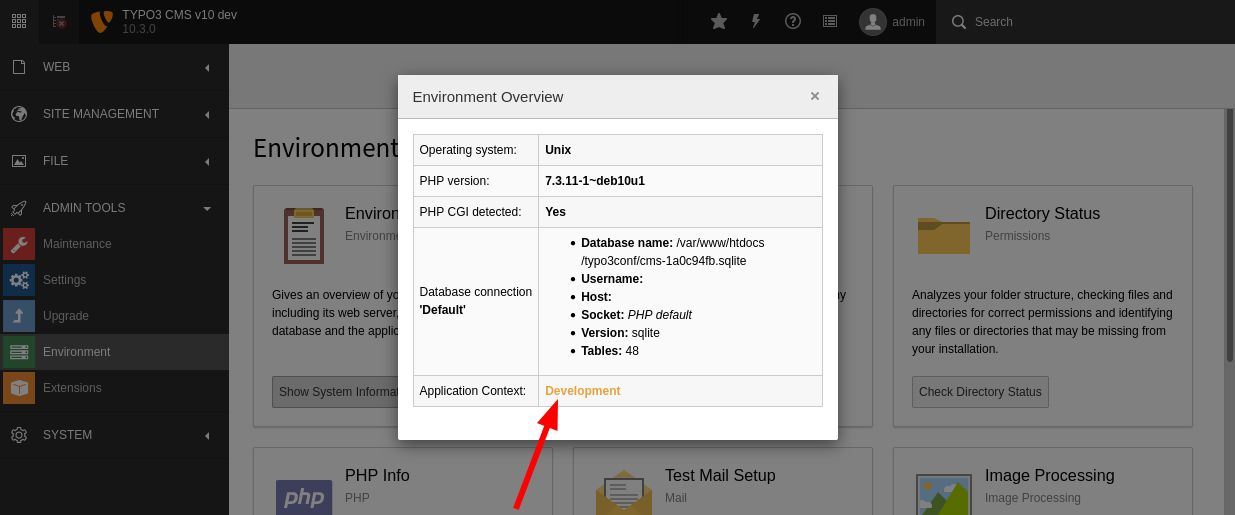
\includegraphics[width=0.9\linewidth]{ChangesForIntegrators/90136-ShowApplicationContextInTheEnvironmentModule.png}
	\end{figure}

\end{frame}

% ------------------------------------------------------------------------------
% Task | 89844 | Improve visual appearance of feature toggles

\begin{frame}[fragile]
	\frametitle{Wijzigingen voor integrators}
	\framesubtitle{Optieschakelaars}

	De weergave van de optieschakelaars is verbeterd:
	\newline\newline
	\smaller\textbf{TYPO3 < 10.3}\tabto{6cm}\textbf{TYPO3 >= 10.3}\normalsize

	\begin{figure}
		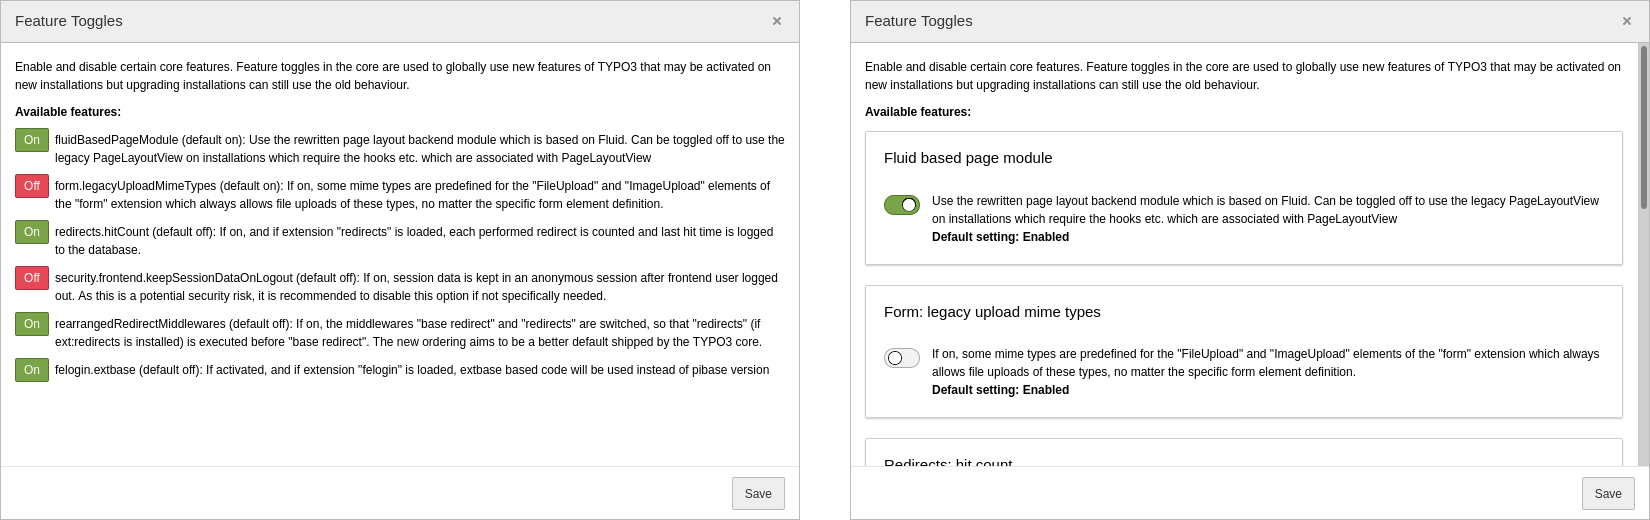
\includegraphics[width=1\linewidth]{ChangesForIntegrators/89844-ImproveVisualAppearanceOfFeatureToggles.png}
	\end{figure}

\end{frame}

% ------------------------------------------------------------------------------
% Feature | 89513 | Provide password recovery for backend users
%
%\begin{frame}[fragile]
%	\frametitle{Wijzigingen voor integrators}
%	\framesubtitle{Password Recovery Email}
%
%	\begin{itemize}
%
%		\item Password resets for backend users are only valid for 4 hours.\newline
%			This time limit is not configurable.
%		\item The function can optionally be disabled for all users or for admin users only to strengthen security.
%		\item If users share one email address, an alternative email text is used.
%		\item TCA field \texttt{be\_users.email} must not be set to \texttt{eval=email}.
%
%		\item The function only works for users, who:
%			\begin{itemize}
%				\item have an email address set,
%				\item have a password set, and
%				\item are not disabled/deleted.
%			\end{itemize}
%
%	\end{itemize}
%
%\end{frame}
%
% ------------------------------------------------------------------------------
